\documentclass[../../report.tex]{subfiles}

\newcommand{\dominatedResult}{
\begin{pmatrix} 
0.151881422 \\
0.106646453 \\
0.0676301244 \\
0.113485461 \\
0.160905627 \\
0.187885977 \\
0.0859075715 \\
0.0696112425 \\
0.10119529 \\
0.055653586
\end{pmatrix}}

\newcommand{\randomResult}{
\begin{pmatrix} 
0.248430651 \\ 
-0.617896379 \\
0.27675287 \\
0.564193533 \\
0.528634855 \\
0.967365431 \\
0.46685821 \\
0.29630525 \\
0.213863252 \\
-0.262269939
\end{pmatrix}
}

\newcommand{\hilbertResult}{
\begin{pmatrix} 
-6.2624771 \\
31.0389149 \\
-8.94248913 \\
-16.873137 \\
-35.113627 \\
-46.62674 \\
11.4857659 \\
52.0688052 \\
33.0079033 \\
15.6151721
\end{pmatrix}
}


\let\dominatedGauss\dominatedResult
\let\dominatedResult\undefined

\let\randomGauss\randomResult
\let\randomResult\undefined

\let\hilbertGauss\hilbertResult
\let\hilbertResult\undefined

\newcommand{\dominatedResult}{
\begin{pmatrix} 
0.151881422 \\
0.106646453 \\
0.0676301244 \\
0.113485461 \\
0.160905627 \\
0.187885977 \\
0.0859075715 \\
0.0696112425 \\
0.10119529 \\
0.055653586
\end{pmatrix}}

\newcommand{\randomResult}{
\begin{pmatrix} 
0.248430651 \\ 
-0.617896379 \\
0.27675287 \\
0.564193533 \\
0.528634855 \\
0.967365431 \\
0.46685821 \\
0.29630525 \\
0.213863252 \\
-0.262269939
\end{pmatrix}
}

\newcommand{\hilbertResult}{
\begin{pmatrix} 
-6.2624771 \\
31.0389149 \\
-8.94248913 \\
-16.873137 \\
-35.113627 \\
-46.62674 \\
11.4857659 \\
52.0688052 \\
33.0079033 \\
15.6151721
\end{pmatrix}
}


\let\dominatedJacobi\dominatedResult
\let\dominatedResult\undefined

\let\randomJacobi\randomResult
\let\randomResult\undefined

\let\hilbertJacobi\hilbertResult
\let\hilbertResult\undefined

\newcommand{\dominatedResult}{
\begin{pmatrix} 
0.151881422 \\
0.106646453 \\
0.0676301244 \\
0.113485461 \\
0.160905627 \\
0.187885977 \\
0.0859075715 \\
0.0696112425 \\
0.10119529 \\
0.055653586
\end{pmatrix}}

\newcommand{\randomResult}{
\begin{pmatrix} 
0.248430651 \\ 
-0.617896379 \\
0.27675287 \\
0.564193533 \\
0.528634855 \\
0.967365431 \\
0.46685821 \\
0.29630525 \\
0.213863252 \\
-0.262269939
\end{pmatrix}
}

\newcommand{\hilbertResult}{
\begin{pmatrix} 
-6.2624771 \\
31.0389149 \\
-8.94248913 \\
-16.873137 \\
-35.113627 \\
-46.62674 \\
11.4857659 \\
52.0688052 \\
33.0079033 \\
15.6151721
\end{pmatrix}
}


\let\dominatedSeidel\dominatedResult
\let\dominatedResult\undefined

\let\randomSeidel\randomResult
\let\randomResult\undefined

\let\hilbertSeidel\hilbertResult
\let\hilbertResult\undefined

\newcommand{\dominatedResult}{
\begin{pmatrix} 
0.151881422 \\
0.106646453 \\
0.0676301244 \\
0.113485461 \\
0.160905627 \\
0.187885977 \\
0.0859075715 \\
0.0696112425 \\
0.10119529 \\
0.055653586
\end{pmatrix}}

\newcommand{\randomResult}{
\begin{pmatrix} 
0.248430651 \\ 
-0.617896379 \\
0.27675287 \\
0.564193533 \\
0.528634855 \\
0.967365431 \\
0.46685821 \\
0.29630525 \\
0.213863252 \\
-0.262269939
\end{pmatrix}
}

\newcommand{\hilbertResult}{
\begin{pmatrix} 
-6.2624771 \\
31.0389149 \\
-8.94248913 \\
-16.873137 \\
-35.113627 \\
-46.62674 \\
11.4857659 \\
52.0688052 \\
33.0079033 \\
15.6151721
\end{pmatrix}
}


\let\dominatedSeidelRel\dominatedResult
\let\dominatedResult\undefined

\let\randomSeidelRel\randomResult
\let\randomResult\undefined

\let\hilbertSeidelRel\hilbertResult
\let\hilbertResult\undefined

\newcommand{\dominatedResult}{
\begin{pmatrix} 
0.151881422 \\
0.106646453 \\
0.0676301244 \\
0.113485461 \\
0.160905627 \\
0.187885977 \\
0.0859075715 \\
0.0696112425 \\
0.10119529 \\
0.055653586
\end{pmatrix}}

\newcommand{\randomResult}{
\begin{pmatrix} 
0.248430651 \\ 
-0.617896379 \\
0.27675287 \\
0.564193533 \\
0.528634855 \\
0.967365431 \\
0.46685821 \\
0.29630525 \\
0.213863252 \\
-0.262269939
\end{pmatrix}
}

\newcommand{\hilbertResult}{
\begin{pmatrix} 
-6.2624771 \\
31.0389149 \\
-8.94248913 \\
-16.873137 \\
-35.113627 \\
-46.62674 \\
11.4857659 \\
52.0688052 \\
33.0079033 \\
15.6151721
\end{pmatrix}
}


\let\dominatedGrad\dominatedResult
\let\dominatedResult\undefined

\let\randomGrad\randomResult
\let\randomResult\undefined

\let\hilbertGrad\hilbertResult
\let\hilbertResult\undefined

\newcommand{\noConvergence}{
  \begin{tabular}[x]{@{}c@{}}Нет\\сходимости\end{tabular}}

\begin{document}

\chapter{Результаты}

\section{Результаты расчетов}
    Приведём здесь записанные подряд векторы, которые были получены в результате работы метода на каждой матрице.
    Также сравним евклидову норму разности вектора свободных членов и вектора, который получается в результате умножения на матрицу итогового ответа каждого метода.

\subsection{Матрица с диагональным преобладанием}
\begin{tabular}{|c|c|c|c|c|}
\hline
Метод Гаусса & Метод Якоби & Метод Зайделя & Метод Зайделя 2 & Метод спуска\\
\hline
$ \dominatedGauss $
  &
$ \dominatedJacobi $
  &
$ \dominatedSeidel $
  &
$ \dominatedSeidelRel $
  &
$ \dominatedGrad $ \\
\hline
\multicolumn{5}{|c|}{Норма разности с ответом}\\
\hline
$0$ & $0.00000135202$ & $0.00000423463$ & $0.00001623736$ & $0.00000000046$ \\
\hline
\multicolumn{5}{|c|}{Количество итераций до завершения}\\
\hline
- & 84 & 20 & 55 & 11 \\
\hline
\end{tabular}
\\

\subsection{Случайная матрица}

\begin{tabular}{|c|c|c|c|c|}
\hline
Метод Гаусса & Метод Якоби & Метод Зайделя & Метод Зайделя 2 & Метод спуска\\
\hline
$ \randomGauss $
  &
  \noConvergence
  &
$ \randomSeidel $
  &
  \noConvergence
  &
$ \randomGrad $ \\
\hline
\multicolumn{5}{|c|}{Норма разности с ответом}\\
\hline
$0$ & - & $0.00103018051$ & - & $0.00000000094$ \\
\hline
\multicolumn{5}{|c|}{Количество итераций до завершения}\\
\hline
- & - & 414 & - & 12 \\
\hline
\end{tabular}

\subsection{Матрица Гильберта}

\begin{tabular}{|c|c|c|c|c|}
\hline
Метод Гаусса & Метод Якоби & Метод Зайделя & Метод Зайделя 2 & Метод спуска\\
\hline
$ \hilbertGauss $
  &
  \noConvergence
  &
$ \hilbertSeidel $
  &
  \noConvergence
  &
$ \hilbertGrad $ \\
\hline
\multicolumn{5}{|c|}{Норма разности с ответом}\\
\hline
$0$ & - & $0.00001438651$ & - & $0.00000004757$ \\
\hline
\multicolumn{5}{|c|}{Количество итераций до завершения}\\
\hline
- & - & 1000 & - & 15 \\
\hline
\end{tabular} \\

\section{Графики}
Итерационные методы различаются скоростью сходимости.
Следующие графики изображают изменение нормы разности вектора $Ax_i - b$ в зависимости от итерации.

\subsection{Матрица с диагональным доминированием}
\begin{center}
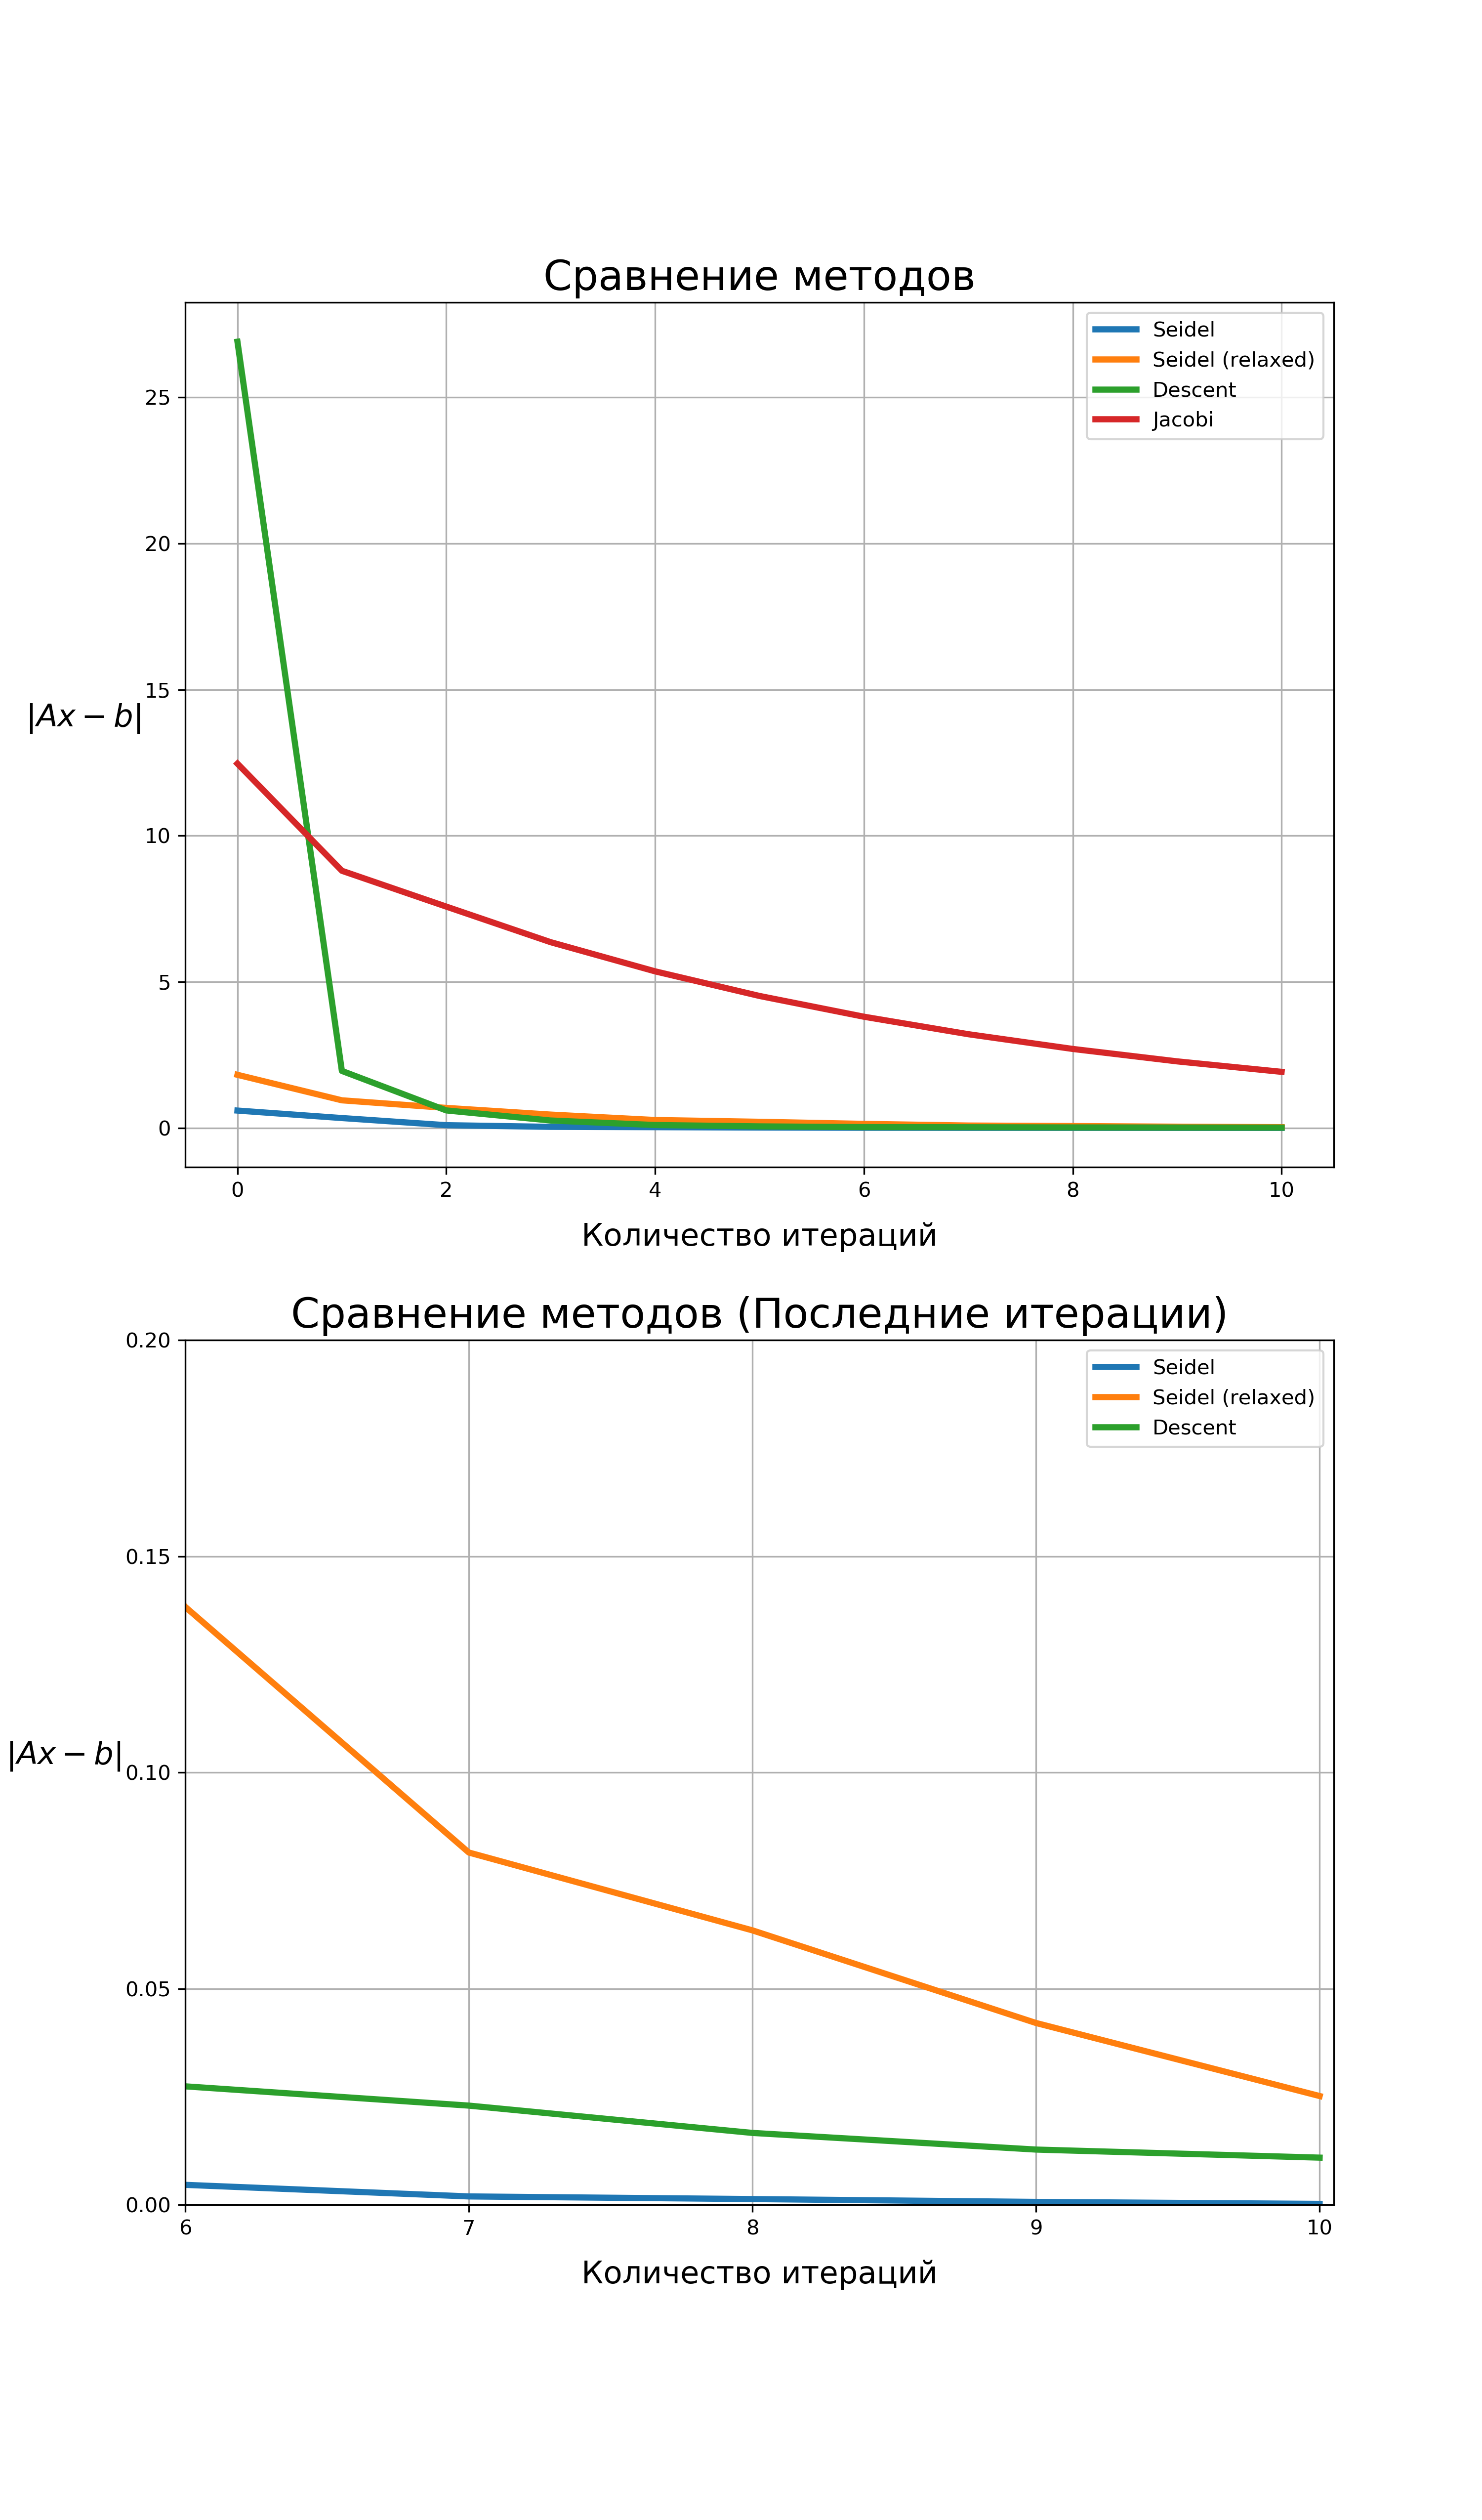
\includegraphics[scale=0.5]{../../../vis/graphs/dominatedNew.png}
\end{center}

\subsection{Случайная матрица}
\begin{center}
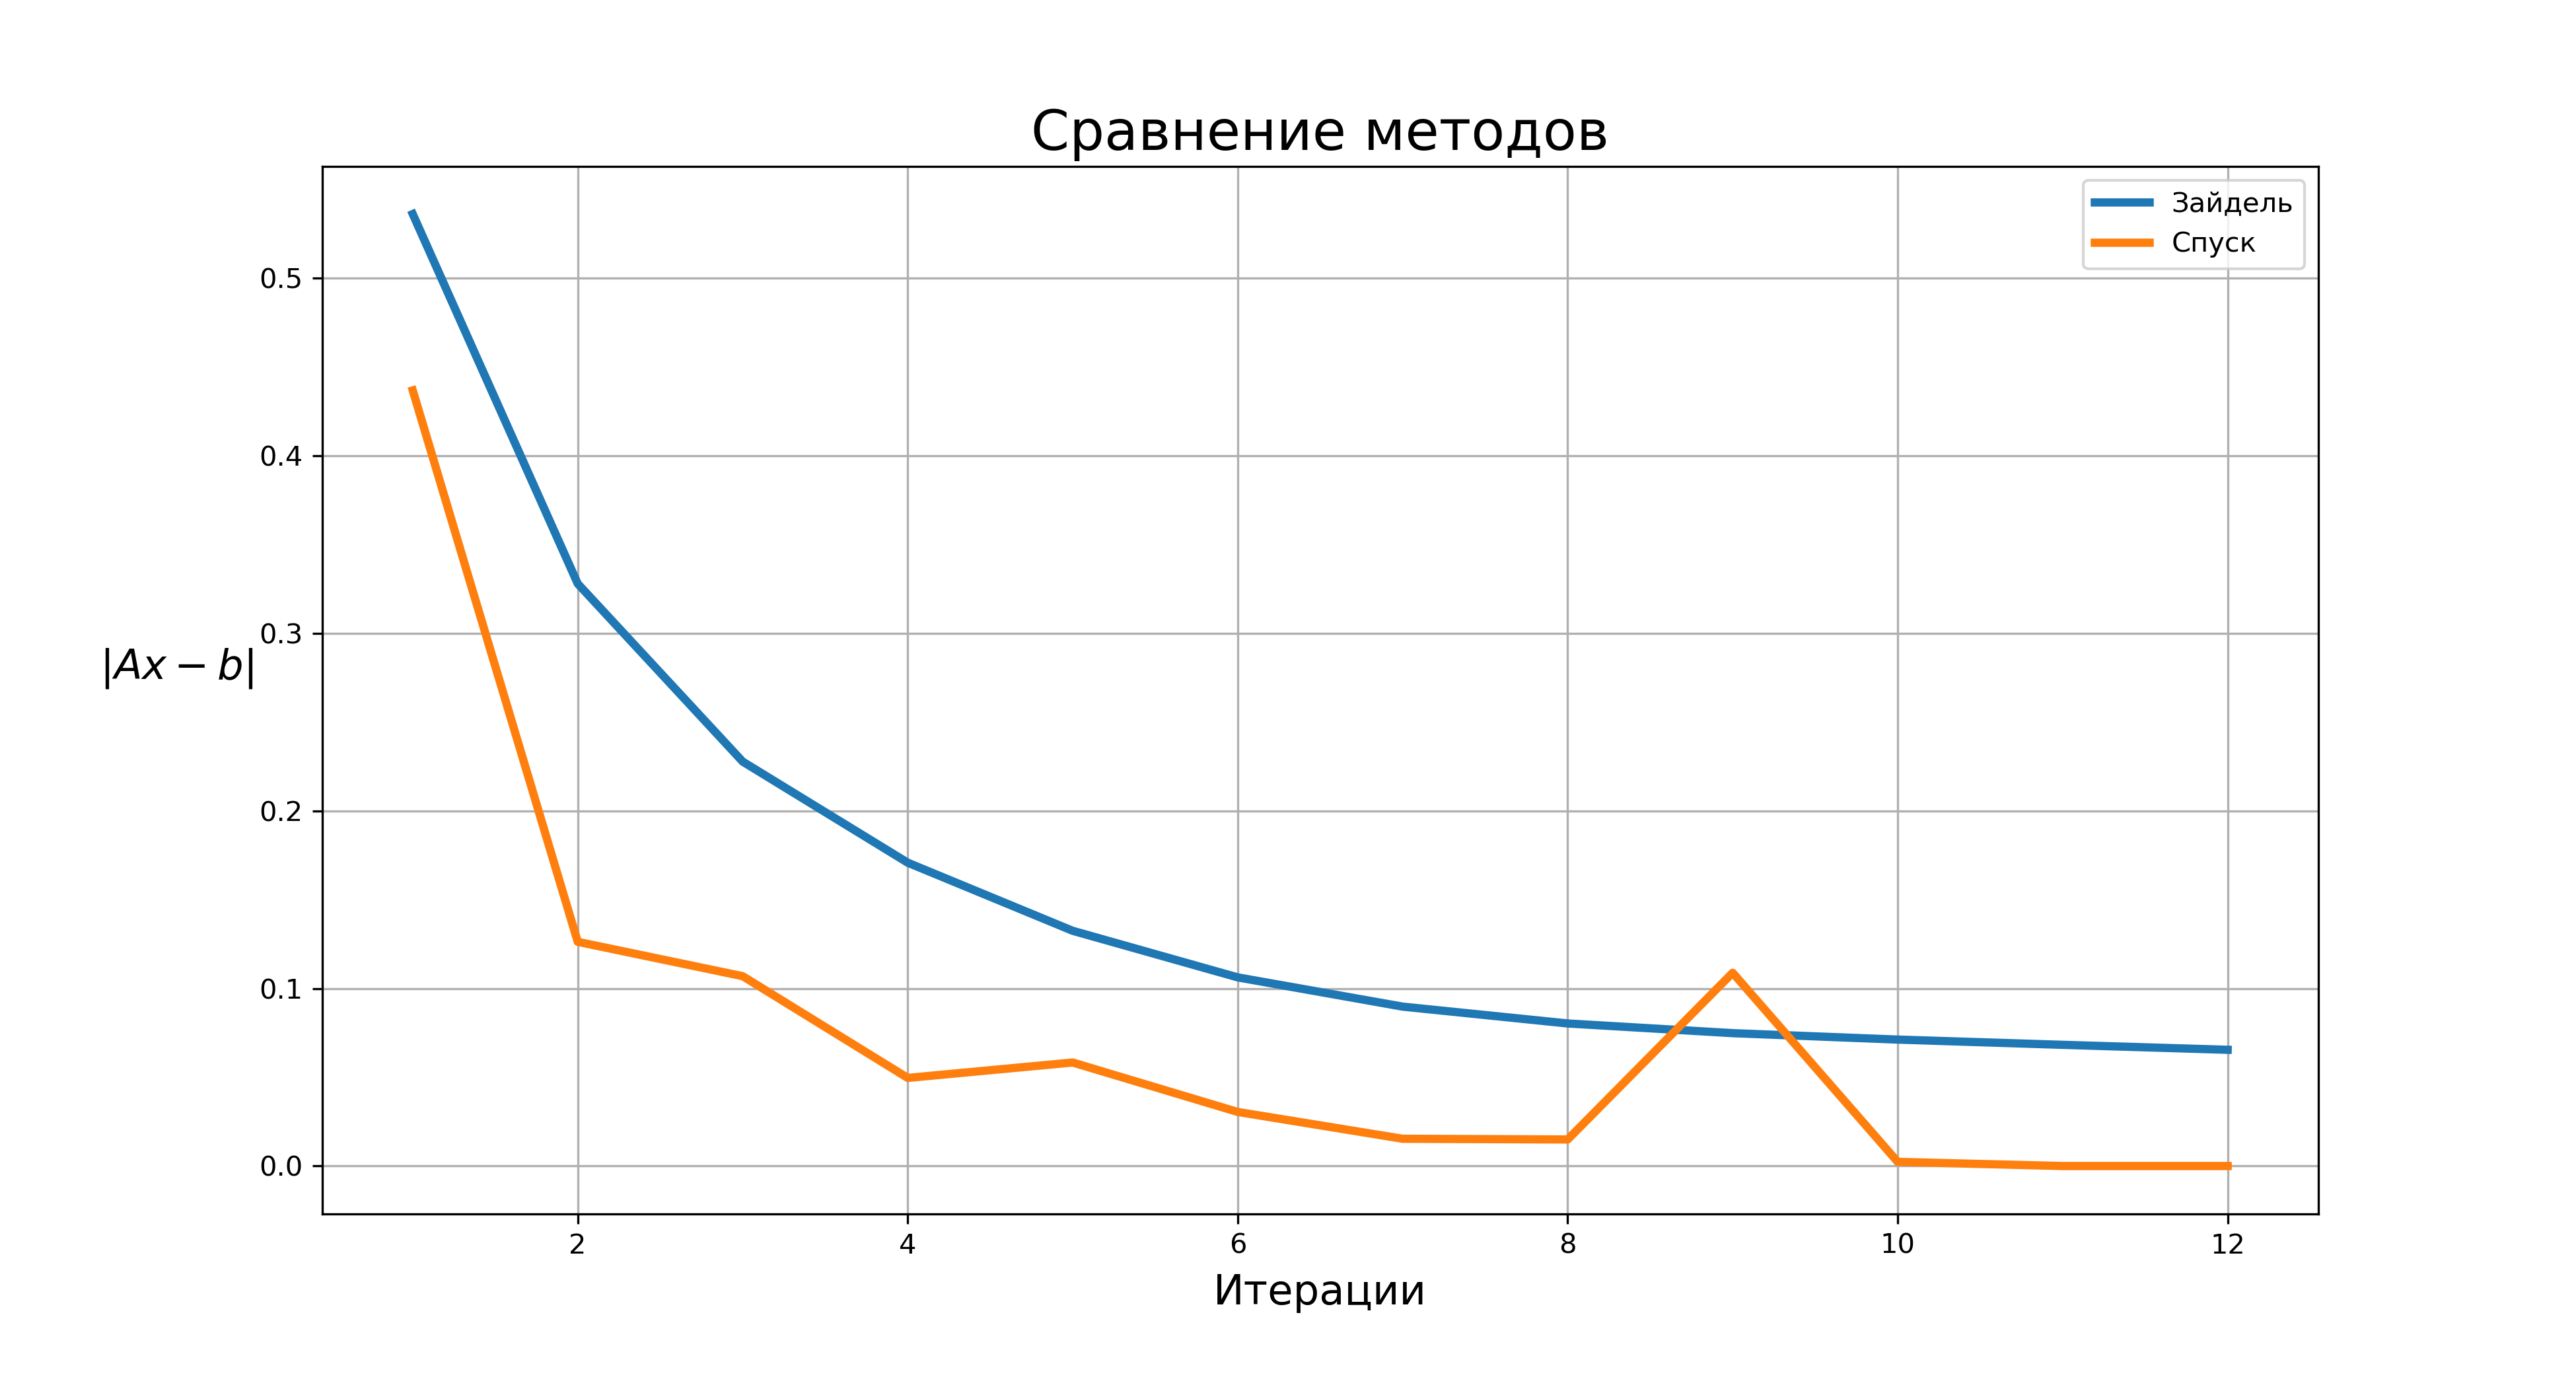
\includegraphics[scale=0.5]{../../../vis/graphs/randomNew.png}
\end{center}

\subsection{Матрица Гильберта}
\begin{center}
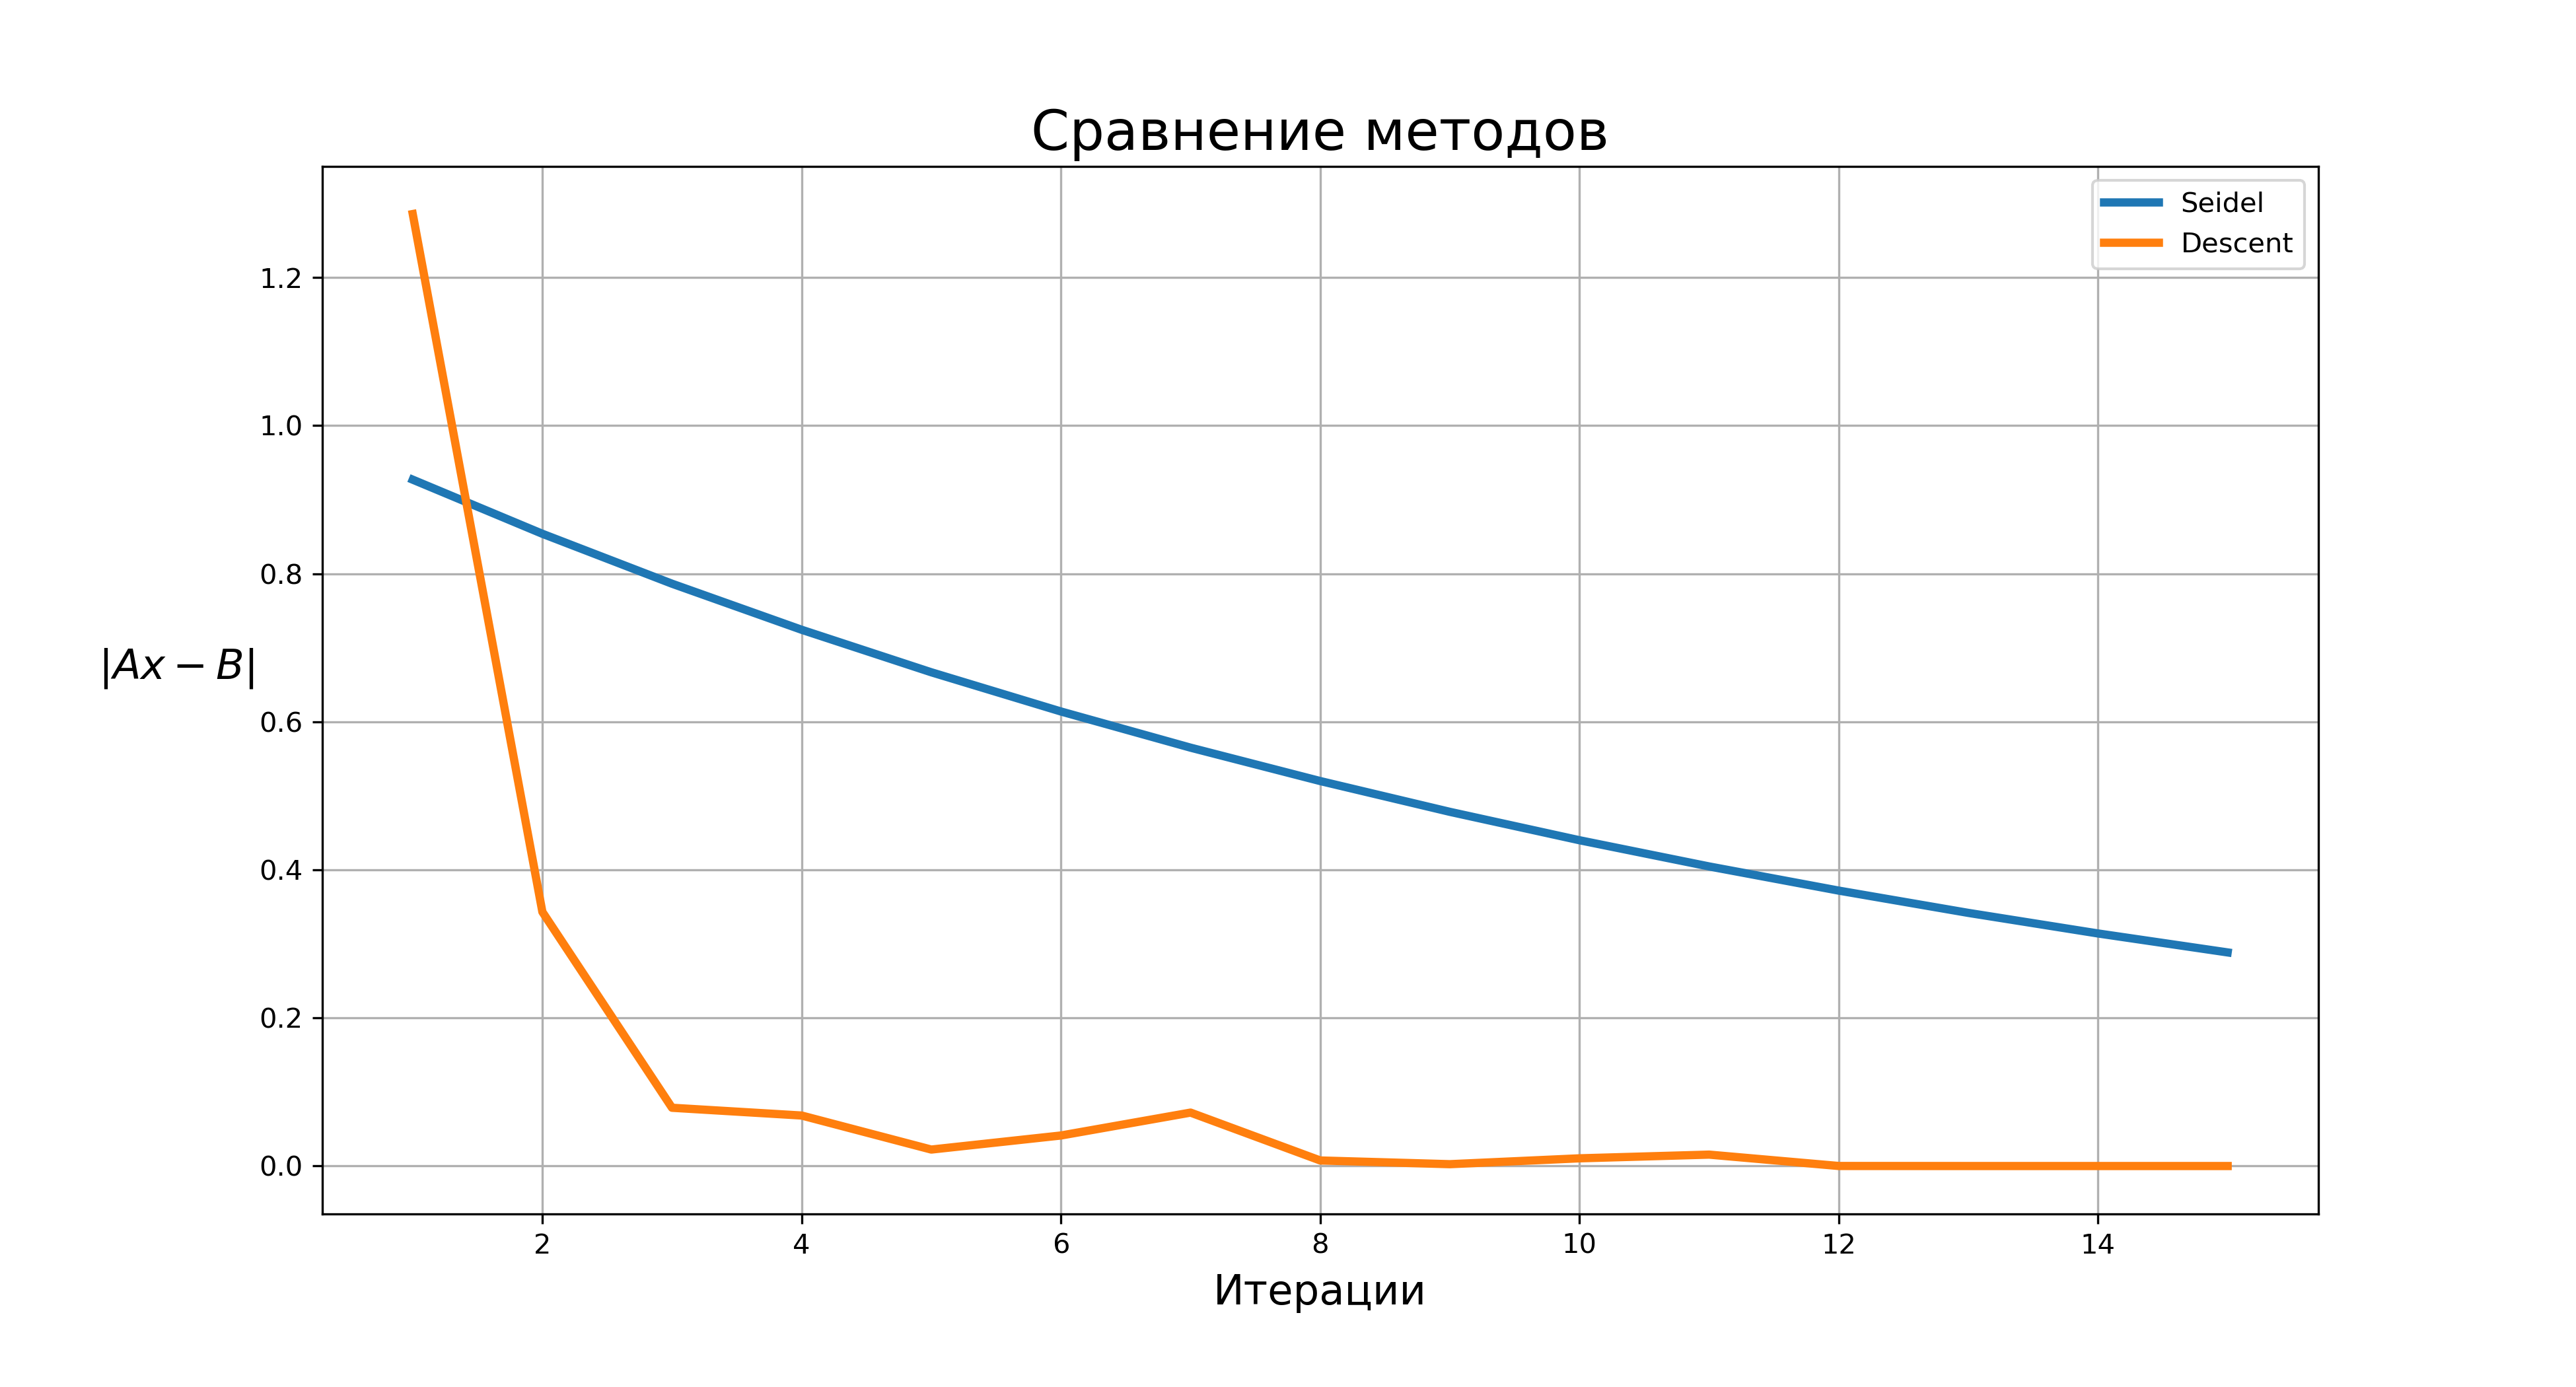
\includegraphics[scale=0.5]{../../../vis/graphs/hilbertNew.png}
\end{center}

\end{document}
